% StateScout AI -- research paper draft
% Build:  cd docs/report/paper && make      (pdflatex + bibtex, see Makefile)
\documentclass[10pt,twocolumn,letterpaper]{article}

\usepackage[margin=0.75in,columnsep=0.25in]{geometry}
\usepackage[T1]{fontenc}
\usepackage{mathptmx}
\usepackage[scaled=0.9]{helvet}
\usepackage{courier}
\usepackage{amsmath,amssymb,amsthm}
\usepackage{microtype}
\usepackage{booktabs,multirow,threeparttable}
\usepackage{graphicx}
\usepackage{xcolor}
\usepackage{tikz}
\usetikzlibrary{arrows.meta,positioning,fit,backgrounds,calc,shapes.geometric}
\usepackage{pgfplots}
\pgfplotsset{compat=1.18}
\usepackage[font=small,labelfont=bf]{caption}
\usepackage{subcaption}
\usepackage{enumitem}
\usepackage[numbers,sort&compress]{natbib}
\usepackage{balance}
\usepackage[colorlinks=true,linkcolor=blue!50!black,citecolor=green!40!black,urlcolor=blue!50!black]{hyperref}
\usepackage[capitalise,nameinlink]{cleveref}

\setlist{nosep,leftmargin=*}
\newtheorem{definition}{Definition}
\newtheorem{proposition}{Proposition}
\newtheorem{corollary}{Corollary}
\newcommand{\sys}{\textsc{StateScout}}
\newcommand{\Forb}{\mathcal{F}}
\newcommand{\Req}{\mathcal{R}}
\newcommand{\Sig}{\Sigma}
\newcommand{\todo}[1]{\textcolor{red!70!black}{[\textbf{TODO:} #1]}}
\definecolor{bad}{HTML}{C0392B}
\definecolor{good}{HTML}{1E7B4F}
\definecolor{mute}{HTML}{7F8C8D}
\definecolor{acc}{HTML}{2E5E8C}

\title{\sys: Auditing What Must \emph{Not} Exist --- Policy-Aware,\\
Negation-Grounded Exploration of Web User Interfaces}

\author{Team 46\thanks{Author names and ordering to be finalised by the team.}\\
Department of Computer Science and Engineering\\
Amrita Vishwa Vidyapeetham\\
\small\textit{Research draft --- \today}}

\date{}

\begin{document}
\maketitle

\begin{abstract}
Web applications enforce authorization on the server, yet their user
interfaces routinely expose what a role should never see: an Admin link
rendered for guests, a debug panel shipped to production, a destructive
control two clicks from the landing page. Such defects evade workflow tests,
because nobody writes a test for a button that is not supposed to exist. We
present \sys{}, an autonomous auditor that explores a web application as a
fixed role and checks every reached UI state against a role-scoped declarative
policy. We make three contributions. (1)~A \emph{polarity-typed policy oracle}
that treats \emph{forbidden-present} ($S\cap\mathcal F$) and
\emph{required-absent} ($\mathcal R\setminus S$) as distinct set operations over
a semantic abstraction of each state. (2)~An \emph{error-direction asymmetry}
result: under-reporting perception can only miss forbidden elements and can
only raise false alarms on required ones, and over-reporting does the reverse.
No single perception bias is therefore safe for both clause types, which
motivates a negation-safe design in which deterministic DOM and
accessibility-tree evidence decides existence and a vision-language model only
annotates. (3)~A \emph{side-effect-aware, cyclic exploration loop} with
claim-before-execute semantics per $(\text{state},\text{action})$ pair,
content-addressed actions, and normalized state fingerprints, implemented as a
checkpointable LangGraph state machine. On a ground-truth application with six
states, four cycles, and four planted violations, the loop recovers the full
cyclic graph with zero duplicate work and reports exactly the planted
violations when perception is an oracle. Replacing the oracle with the
deterministic perception channel drops precision to 0.29 and recall to 0.50,
with errors that follow the predicted asymmetry exactly. A lexical-grounding
ablation restores precision to 1.00 but not recall, which isolates
\emph{semantic subject grounding} as the open problem. State normalization
collapses 300 noisy captures to the 6 true states while still separating a
state that gains or loses a Delete button.
\end{abstract}

\section{Introduction}
\label{sec:intro}

Broken access control heads the OWASP Top~10~\cite{owasp2021a01}. Most
research tools for it ask whether the \emph{server} enforces authorization,
by comparing or replaying requests under different identities
\cite{sun2011static,li2014blackbox,noseevich2011detecting,monshizadeh2014mace,liu2025bacscan}.
A related class of defect lives one layer up. Consider a dashboard that
renders an \emph{Admin} link for every role. The backend correctly rejects a
guest's request, so a request-level scanner reports nothing. The link itself
still leaks the existence and location of privileged functionality, invites
probing, and violates the organisation's least-privilege UI policy. The same
applies to a debug panel left in a production build, a destructive control a
guest can reach in two clicks, or the \emph{absence} of an element the policy
requires, such as a skip-to-content link, a consent banner, or a logout
affordance.

Workflow-based UI testing does not catch these defects, because tests check
what \emph{should} happen and nobody writes a test for a button that should
not exist. Model-inference crawlers~\cite{mesbah2012crawljax,memon2003ripping,dallmeier2013webmate}
explore autonomously but check generic or hand-coded invariants. DOM
invariants~\cite{mesbah2012invariant} can express presence and absence, but as
per-page XPath predicates written in code, with no notion of role. LLM and
VLM GUI agents~\cite{liu2024gptdroid,yoon2024droidagent,liu2024visiondroid,zheng2024seeact}
explore or judge screens in natural language, but they let a model issue the
verdict, which is risky when the verdict is ``this element is \emph{not}
there'': VLMs are known to handle negation poorly~\cite{alhamoud2025negation}.

\paragraph{This paper.}
We present \sys{}, which reframes UI testing as \emph{state-space auditing}.
Given a seed URL, a role, and a policy of the form ``a guest must never see the
admin link; every page must offer a skip-to-content link'', \sys{} explores the
application autonomously, keeps the full cyclic state graph, and audits every
reached state. Each finding carries the policy clause it breaks, the set
operation that caught it, and human-checkable evidence.

\paragraph{Contributions.}
We do not claim to be the first to crawl web applications into state graphs,
to check invariants on crawled states, or to use VLMs for GUI testing; each has
substantial prior art (\cref{sec:related}). Our contributions are a
formalisation and a design that \emph{combine} these threads for a question
none of them targets: \emph{does the UI a given role can reach conform to a
declared policy of what must and must not exist?}
\begin{enumerate}
  \item \textbf{A polarity-typed, role-scoped policy oracle}
    (\cref{sec:model}). Forbidden-present ($S\cap\mathcal F$) and
    required-absent ($\mathcal R\setminus S$) are distinct set operations over
    a \emph{semantic} state abstraction (roles, accessible names, tags,
    capabilities), not raw XPath. Polarity is part of the policy schema, and
    every violation is tagged with its clause type.
  \item \textbf{An error-direction asymmetry result}
    (\cref{prop:asym}) together with its empirical confirmation
    (\cref{sec:eval:rq2}). Perception errors propagate in opposite directions
    for the two clause types. This argues for reporting accuracy \emph{per
    polarity} and for a \emph{negation-safe division of labour}, in which
    deterministic DOM/AX evidence decides existence and a VLM only annotates.
  \item \textbf{A side-effect-aware cyclic exploration loop}
    (\cref{sec:system}). It uses claim-before-execute per $(v,a)$ pair,
    kind-restricted replay, content-addressed actions, and normalized
    fingerprints, and runs as a checkpointable LangGraph state machine behind
    typed ports.
  \item \textbf{An honest, reproducible evaluation} on a polarity-complete
    ground-truth application (\cref{sec:eval}). It separates what the loop
    guarantees (exact recovery with an oracle perceiver) from what perception
    currently delivers, and localizes the remaining gap to semantic subject
    grounding.
\end{enumerate}

Unlike access-control scanners, \sys{} does not test server-side enforcement.
It audits what each role \emph{sees}, so the two are complementary.

\section{Motivating Example}
\label{sec:background}

\Cref{fig:app} (\cref{sec:eval}) shows \texttt{broken-admin}, a six-page
application built as ground truth. A guest lands on \texttt{index}, signs in,
and reaches \texttt{dashboard}. From there the guest can open
\texttt{reports} and \texttt{admin}, and every page links back. The policy,
written in English and stored with its structured form, reads:

\begin{quote}\small
(F1) A guest must never see the admin link.
(F2) A guest must never be able to delete a user.
(F3) No page may ship a debug panel.
(R1) Every page must offer a skip-to-content link.
\end{quote}

Four violations are planted. The Admin link on \texttt{dashboard} breaks F1.
The debug panel on \texttt{reports} breaks F3. The Delete-user button on
\texttt{admin} breaks F2. \texttt{admin} is also the only page without a
skip-to-content link, which breaks R1.

Three observations follow from this example. \emph{First}, no workflow test
catches F1--F3, because each defect is extra UI, not broken UI. \emph{Second},
R1 is an \emph{absence}. An engine that only intersects what it sees with a
forbidden list cannot express it (\cref{sec:eval:rq3}). \emph{Third}, the
graph is dense with cycles (log out, back to dashboard). A crawler that drops
back-edges still ``finds the violations'' but throws away the navigation
evidence that a path-sensitive policy (``reachable without signing in'') would
need.

\section{Problem Formulation}
\label{sec:model}

\subsection{Applications, roles, and observations}

We model a web application under test (AUT), as seen by a fixed role $r$, as a
labelled transition system $M_r=(Q,A,\delta,q_0)$ over concrete UI
configurations $Q$, actions $A$, and a partial transition function
$\delta:Q\times A\rightharpoonup Q$. The auditor never sees $Q$ directly. A
\emph{capture} $\kappa(q)=(u,d,t,s)$ bundles the URL, serialized DOM,
accessibility (AX) tree, and an optional screenshot. \sys{} pins one role per
run; multi-role coverage is several runs, and comparing roles is a
reporting-layer concern (\cref{sec:discussion}).

\begin{definition}[State abstraction]
A \emph{fingerprint} is $\phi = H\circ N$, where $N$ normalizes a capture by
removing volatile content (session and CSRF tokens, nonces, long numeric
timestamps, generated hex identifiers, per-session CDP node ids, transient
focus), and $H$ is SHA-256. Two configurations are \emph{the same abstract
state} iff $\phi(\kappa(q))=\phi(\kappa(q'))$.
\end{definition}

Normalization has two failure modes. If it is too sensitive, the model
explodes into one node per page load. If it is too coarse, a security-relevant
change (for example, a destructive button that appears) folds into an existing
state and is never audited. \Cref{sec:eval:fp} measures both.

\subsection{The exploration graph is cyclic}

\begin{definition}[Exploration graph]
The \emph{exploration graph} is a directed multigraph $G=(V,E)$ with
$V\subseteq\operatorname{img}\phi$ and $E\subseteq V\times A\times V$, where
$(v,a,v')\in E$ records that executing $a$ in $v$ was observed to lead to $v'$.
An edge is a \emph{back-edge} if $v'$ was already discovered when it was added.
\end{definition}

Model-inference crawlers often treat revisits as redundant and drop them,
leaving a tree or DAG. We treat back-edges as \emph{evidence}. ``Log out
returns to login'' and ``Admin returns to Dashboard'' are facts about the
AUT's navigation structure, and a path-sensitive audit can only reason over
them if they are kept. \sys{} therefore never prunes an edge. Loop prevention
lives entirely in a \emph{claim set} $C\subseteq V\times A$.

\begin{definition}[Claim-before-execute]
Action $a$ is executed from $v$ only if $(v,a)\notin C$, and $(v,a)$ is inserted
into $C$ \emph{before} $a$ is sent to the browser. The edge $(v,a,v')$ is
persisted only \emph{after} $a$ succeeds.
\end{definition}

\begin{proposition}[Termination and at-most-once per pair]
\label{prop:term}
Suppose $|V|\le n$, which is enforced by a state cap, and each state enables
at most $k$ actions. Then exploration performs at most $nk$ \emph{frontier}
executions and terminates. No claimed pair $(v,a)$ is executed as a frontier
action twice, including across crash and resume.
\end{proposition}
\begin{proof}[Proof sketch]
Every frontier execution inserts a distinct pair into $C$ first, and
$|C|\le nk$. On resume, a pair that is in $C$ but has no edge is treated as
done and never re-fired. Execution strictly follows insertion, so a crash
cannot cause a second execution of the same pair.
\end{proof}

Most AUTs are not idempotent: re-submitting a form changes the application
being audited. Reaching a queued action with a single browser, however, means
\emph{replaying} its path from the seed, and replay re-fires the actions on
that path. \Cref{prop:term} is therefore a guarantee about \emph{pairs}, not
about \emph{effects}. \sys{} narrows the gap by kind: only
$\textsf{ReplaySafe}=\{\texttt{navigate},\texttt{click},\texttt{back}\}$ may be
re-fired. A candidate whose path passes through a \texttt{fill},
\texttt{select}, or \texttt{submit} is recorded as skipped, with a reason, and
its subtree is reported as unexplored instead of being reached by quietly
re-submitting a form. The residual assumption is that \emph{clicks are
navigational}. A click that mutates state on a replayed path (for example, a
one-click ``Delete'') \emph{is} re-fired. We treat this as an open limitation
(\cref{sec:discussion}), not a solved problem. Action identity is
\emph{content-addressed}:
$\mathit{id}(a)=H(\mathit{role}\,\|\,\mathit{name}\,\|\,\mathit{selector})$, not
a DOM index. Replay therefore survives DOM reordering, and the same ``Log out''
control keeps one identity everywhere, while deduplication stays scoped to
$(v,a)$.

\subsection{Policies as two set operations}

A policy is written in English by a QA engineer and compiled into
machine-checkable clauses $c=(\sigma_c,\rho_c,\pi_c)$: a \emph{subject}
$\sigma_c$ (a UI element kind or capability), a role scope $\rho_c$ (empty
means all roles), and a polarity $\pi_c\in\{\textsf{must\_exist},
\textsf{must\_not\_exist}\}$. This splits the policy into forbidden clauses
$\Forb$ and required clauses $\Req$. Perception maps each state to a set of
grounded subjects $\Sig(v)$ (element tags, accessible names, and capabilities).
For a role $r$, let $\Forb_r$ and $\Req_r$ be the clauses whose scope admits
$r$.

\begin{definition}[Negation-aware audit]
\begin{align}
\mathit{Viol}_\Forb(v) &= \{\,c\in\Forb_r : \sigma_c\in\Sig(v)\,\}
  && \text{(forbidden present)}\label{eq:forb}\\
\mathit{Viol}_\Req(v)  &= \{\,c\in\Req_r : \sigma_c\notin\Sig(v)\,\}
  && \text{(required absent)}\label{eq:req}
\end{align}
The audit of $v$ is $\mathit{Viol}_\Forb(v)\cup\mathit{Viol}_\Req(v)$, and each
violation is tagged with the operation that produced it.
\end{definition}

\Cref{eq:forb} is an intersection ($S\cap\Forb$) and \cref{eq:req} is a
difference ($\Req\setminus S$). No single intersection can express both, so an
intersection-only oracle is structurally unable to report a missing element
(\cref{sec:eval:rq3}).

\subsection{Error-direction asymmetry under imperfect perception}
\label{sec:model:asym}

In a real system, $\Sig(v)$ is replaced by a perception estimate $\hat\Sig(v)$
from a DOM/AX correlator or a vision-language model. The two clause types react
to perception errors in \emph{opposite} directions.

\begin{proposition}[Error-direction asymmetry]
\label{prop:asym}
Let $\widehat{\mathit{Viol}}$ denote the audit computed on $\hat\Sig$.
\begin{enumerate}
  \item If perception \emph{under-reports} ($\hat\Sig(v)\subseteq\Sig(v)$), then
    $\widehat{\mathit{Viol}}_\Forb(v)\subseteq\mathit{Viol}_\Forb(v)$ and
    $\widehat{\mathit{Viol}}_\Req(v)\supseteq\mathit{Viol}_\Req(v)$. Forbidden
    clauses can only be missed, and required clauses can only raise false
    alarms.
  \item If perception \emph{over-reports} ($\hat\Sig(v)\supseteq\Sig(v)$, for
    example by hallucinating a subject), both inclusions reverse.
\end{enumerate}
\end{proposition}
\begin{proof}
\Cref{eq:forb} is monotone in $\Sig$ and \cref{eq:req} is antitone in $\Sig$.
\end{proof}

\begin{corollary}
No uniform perception bias is safe for both clause types. A detector tuned to
avoid false alarms on forbidden clauses (conservative, under-reporting) creates
false alarms on required clauses, and the reverse also holds.
\end{corollary}

This matters for multimodal perception. Vision-language models answer negated
queries close to chance~\cite{alhamoud2025negation}, and their compositional
understanding is known to be shallow~\cite{yuksekgonul2023aro,ma2023crepe}.
Those studies use natural images, not UI screenshots, so we cite them as
motivation rather than as a measurement of UI perception. Whatever a
perceiver's error rate, \cref{prop:asym} shows that a single yes/no ``is
$\sigma$ on the screen?'' query has a polarity-dependent risk profile. This motivates the design
choices in \cref{sec:system:negation}: evidence-carrying verdicts, a
deterministic DOM/AX channel that cross-checks the VLM, and (proposed) a
three-valued verdict that abstains instead of guessing when the two channels
disagree. \Cref{sec:eval:rq2} observes exactly the asymmetry predicted by
\cref{prop:asym}.

\section{The \sys{} System}
\label{sec:system}

\begin{figure*}[t]
\centering
\resizebox{\textwidth}{!}{%
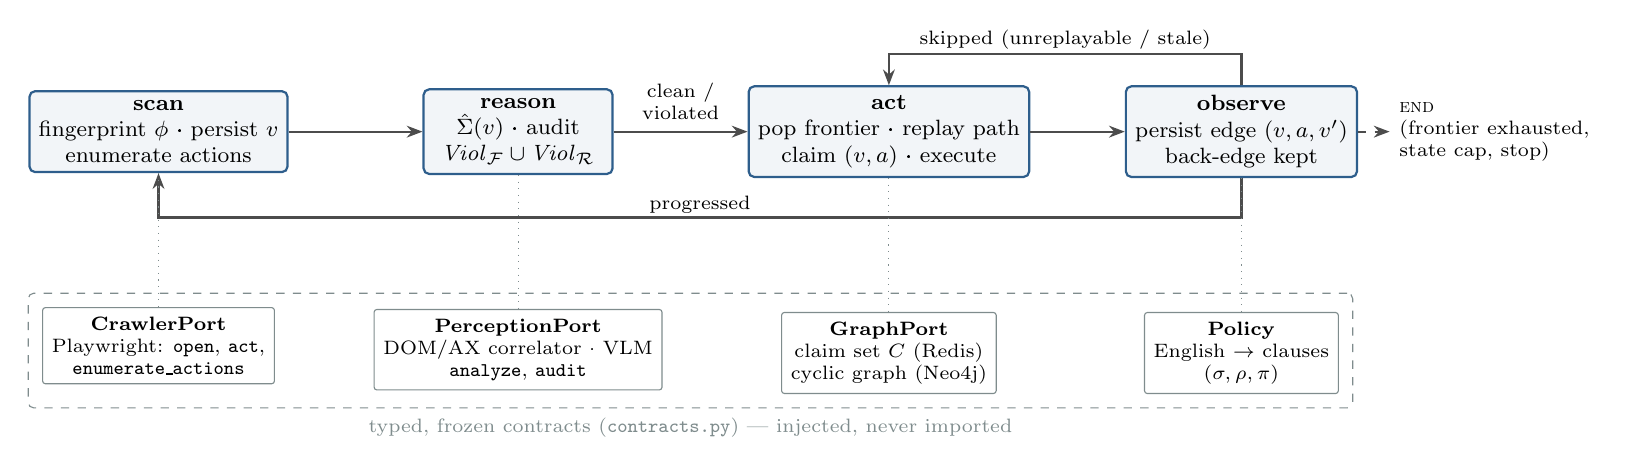
\begin{tikzpicture}[
  font=\footnotesize,
  box/.style={draw=acc,thick,rounded corners=2pt,fill=acc!6,minimum height=9mm,
              minimum width=24mm,align=center},
  port/.style={draw=mute,dashed,rounded corners=2pt,inner sep=5pt},
  data/.style={draw=mute,fill=white,rounded corners=1pt,align=center,font=\scriptsize},
  arr/.style={-{Stealth[length=2mm]},thick,draw=black!70},
  lbl/.style={font=\scriptsize,fill=white,inner sep=1pt}]

  \node[box] (scan)    {\textbf{scan}\\fingerprint $\phi$ · persist $v$\\enumerate actions};
  \node[box,right=17mm of scan] (reason) {\textbf{reason}\\$\hat\Sigma(v)$ · audit\\$\mathit{Viol}_\mathcal F\cup\mathit{Viol}_\mathcal R$};
  \node[box,right=17mm of reason] (act) {\textbf{act}\\pop frontier · replay path\\claim $(v,a)$ · execute};
  \node[box,right=12mm of act] (obs) {\textbf{observe}\\persist edge $(v,a,v')$\\back-edge kept};

  \draw[arr] (scan) -- (reason);
  \draw[arr] (reason) -- node[lbl,above=1mm,align=center]{clean /\\violated} (act);
  \draw[arr] (act) -- (obs);
  \draw[arr] (obs.south) -- ++(0,-5mm) -| node[lbl,pos=0.25,above]{progressed} (scan.south);
  \draw[arr] (obs.north) -- ++(0,4mm) -| node[lbl,pos=0.25,above]{skipped (unreplayable / stale)} (act.north);
  \node[right=4mm of obs,font=\scriptsize,align=left] (end) {\textsc{end}\\(frontier exhausted,\\ state cap, stop)};
  \draw[arr,dashed] (obs) -- (end);

  \node[data,below=17mm of scan]   (crawl) {\textbf{CrawlerPort}\\Playwright: \texttt{open}, \texttt{act},\\\texttt{enumerate\_actions}};
  \node[data,below=17mm of reason] (perc)  {\textbf{PerceptionPort}\\DOM/AX correlator · VLM\\\texttt{analyze}, \texttt{audit}};
  \node[data,below=17mm of act]    (graph) {\textbf{GraphPort}\\claim set $C$ (Redis)\\cyclic graph (Neo4j)};
  \node[data,below=17mm of obs]    (pol)   {\textbf{Policy}\\English $\to$ clauses\\$(\sigma,\rho,\pi)$};

  \begin{scope}[on background layer]
    \node[port,fit=(crawl)(perc)(graph)(pol),label={[font=\scriptsize,text=mute]below:typed, frozen contracts (\texttt{contracts.py}) --- injected, never imported}] {};
  \end{scope}
  \foreach \a/\b in {scan/crawl,reason/perc,act/graph} \draw[-,thin,draw=mute,dotted] (\a) -- (\b);
  \draw[-,thin,draw=mute,dotted] (obs) -- (pol);
\end{tikzpicture}}
\caption{\sys{} architecture. A checkpointed LangGraph state machine of four
nodes and two conditional edges drives the Scan$\to$Reason$\to$Act$\to$Observe
loop. All I/O goes through three typed ports, so every component can be
replaced by a deterministic fake for testing and by the live implementation in
production without changing the loop.}
\label{fig:arch}
\end{figure*}

\Cref{fig:arch} shows the architecture. The implementation consists of about
5.8k lines of Python across five modules owned by four sub-teams, plus a
FastAPI reporting service and a VS~Code extension front-end.

\subsection{Orchestration}
The explorer performs breadth-first search over $(v,a)$ pairs. A plain-Python
reference loop, kept as a \emph{parity oracle}, is ported to a LangGraph
\texttt{StateGraph} with four nodes (\texttt{scan}, \texttt{reason},
\texttt{act}, \texttt{observe}) and two conditional edges. The whole
exploration state (frontier, claimed pairs, discovery order, skips) is a
single checkpointed \texttt{TypedDict}, so a crashed run can resume instead of
restarting. Limits such as depth, state cap, and perception rate are
configuration rather than state, so a resumed run cannot silently run under
different rules. A separate conditional edge routes a skipped action back to
\texttt{act} and not through \texttt{scan}. Otherwise an unchanged state would
be re-audited and a phantom entry added to the discovery order, and the
discovery order is the evidence for cycles. The same test suite runs against
both implementations.

\subsection{Capture and actions}
A Playwright crawler captures DOM, the CDP full AX tree, and a screenshot. It
derives candidate actions from actionable AX roles (link, button, tab,
menuitem, \dots) and gives each one a content-addressed identifier. Navigation
failures and action failures raise distinct exception types, so the
orchestrator can retry the former with backoff and mark-and-skip the latter
without type-sniffing.

\subsection{State abstraction and persistence}
$\phi$ removes known volatile attributes (\texttt{nonce},
\texttt{data-session}, \texttt{data-csrf}, \dots), hex-like generated ids,
prefixed tokens (\texttt{sess\_}, \texttt{csrf\_}, \texttt{tok\_}), 10+-digit
timestamps, whitespace, and volatile CDP keys (\texttt{nodeId},
\texttt{backendDOMNodeId}, \texttt{parentId}, \texttt{childIds}, focus). It
then hashes URL, DOM, and canonical AX JSON together. The claim set lives in
Redis. States, edges (including back-edges), and violations are stored in
Neo4j, where the cyclic structure can be queried directly (for example, ``all
paths from the seed to a violating state'').

\subsection{Perception: grounding subjects in the UI}
\label{sec:system:perception}
Perception turns a capture into a \emph{Semantic UI Map}: elements with role,
accessible name, tags, selector, visibility and enabled state, plus the
capabilities the state exposes (\texttt{delete-user}, \texttt{export-data},
\dots). The baseline channel is deterministic and fully reproducible. It
correlates DOM elements and AX nodes by (i)~browser-provided identifiers,
(ii)~role plus accessible name, and (iii)~name alone when unique. Ambiguous
matches are never guessed. DOM-only elements are kept on purpose, because an
element hidden from the AX tree can still be an exposure. A vision-language
model channel (Gemini~2.5 Flash, behind a rate-limited provider interface)
reads the screenshot and AX tree. It supplies judgements the DOM cannot make,
such as a styled \texttt{<div>} with no ARIA role that \emph{looks like} a
delete button. By design it may only \emph{annotate} elements the
deterministic channel already found, adding tags and capabilities. It may never
add or remove an element, so existence and absence (the polarity that VLMs are
known to handle poorly~\cite{alhamoud2025negation}) are decided by evidence
that cannot be hallucinated. In the current codebase this channel is
implemented but not yet wired into the orchestrator, and it is not evaluated
in this paper. A run without screenshots is labelled a smoke test, not an
audit.

\subsection{Negation engine}
\label{sec:system:negation}
The audit implements \cref{eq:forb,eq:req} deterministically. Clause
applicability is checked against the run's role. Subjects are matched first
against capabilities, which are stronger evidence, and then against element
tags and accessible names. There is no substring matching, because an
over-eager matcher is exactly the over-reporting bias of \cref{prop:asym}.
Every violation carries its clause type, a severity, a plain-language
rationale, and \emph{evidence} (selector, text, screenshot) that a human can
check. The policy compiler that turns English sentences into clauses is
\emph{in progress}. By design it reuses the perception port's text channel, so
there is one model client and one rate limit, and it includes a confirmation
gate on which the QA engineer approves the parse before the crawl. In this
draft, policies are supplied in structured form next to their English source
(\texttt{policy.json}).

\subsection{Ground-truth test applications}
Each test application ships three machine-readable files next to its HTML:
\texttt{app.json} (pages and controls), \texttt{policy.json} (the English
policy and its structured form), and \texttt{violations.json} (every planted
defect with its page and clause). Evaluation asserts \emph{exact} set equality
between found and planted violations. A miss is a regression, and an
undocumented finding is a false positive. A consistency test fails if the HTML
and \texttt{app.json} drift apart.

\section{Evaluation}
\label{sec:eval}

We ask four research questions:
\begin{description}
  \item[RQ1] Does the exploration loop reach every state, keep the graph
    cyclic, avoid duplicate work, and report exactly the planted violations?
  \item[RQ2] How does the perception channel's subject grounding affect audit
    accuracy, and does the error follow \cref{prop:asym}?
  \item[RQ3] Is the required-absent operation (\cref{eq:req}) necessary, or is
    an intersection-only oracle enough?
  \item[RQ4] Is the fingerprint $\phi$ stable under volatile content and still
    sensitive to real UI changes?
\end{description}

\paragraph{Subject application.}
\texttt{broken-admin} is a static six-page application (index, login,
register, dashboard, reports, admin) with four cycles and four planted
violations, browsed as \texttt{guest} (\cref{fig:app}). The policy has three
forbidden clauses (admin link, delete-user, debug panel) and one required
clause (skip-to-content link). V-01 is an Admin link rendered for every role;
the backend rejects the request, but the link itself is the exposure. V-02 is
a debug panel left in the production build. V-03 is a Delete-user control two
clicks from the seed. V-04 is a missing skip-to-content link, which is an
\emph{absence}.

\paragraph{Reproducibility.}
All numbers are produced by
\nolinkurl{docs/demo_crawl.py} (RQ1) and
\nolinkurl{docs/report/experiments/run_experiments.py} (RQ2--RQ4). The raw
output is in \nolinkurl{docs/report/data/experiments.json}. Every run is
deterministic.

\begin{figure}[t]
\centering
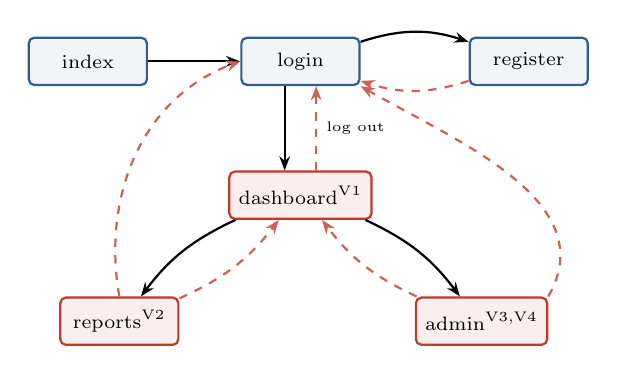
\begin{tikzpicture}[font=\scriptsize,
  st/.style={draw=acc,thick,rounded corners=2pt,fill=acc!6,minimum width=15mm,minimum height=6mm},
  vio/.style={st,draw=bad,fill=bad!8},
  fe/.style={-{Stealth[length=1.8mm]},thick},
  be/.style={-{Stealth[length=1.8mm]},thick,dashed,draw=bad!80}]
  \node[st]  (idx) at (0,0)      {index};
  \node[st]  (log) at (2.7,0)    {login};
  \node[st]  (reg) at (5.6,0)    {register};
  \node[vio] (das) at (2.7,-1.7) {dashboard$^{\text{V1}}$};
  \node[vio] (rep) at (0.4,-3.3) {reports$^{\text{V2}}$};
  \node[vio] (adm) at (5.0,-3.3) {admin$^{\text{V3,V4}}$};
  \draw[fe] (idx) -- (log);
  \draw[fe] (log) to[bend left=18] (reg);
  \draw[be] (reg) to[bend left=18] (log);
  \draw[fe] ([xshift=-2mm]log.south) -- ([xshift=-2mm]das.north);
  \draw[be] ([xshift=2mm]das.north) -- node[right,font=\tiny]{log out} ([xshift=2mm]log.south);
  \draw[fe] (das) to[bend right=14] (rep);
  \draw[be] (rep) to[bend right=14] (das);
  \draw[fe] (das) to[bend left=14] (adm);
  \draw[be] (adm) to[bend left=14] (das);
  \draw[be] (rep.north) to[out=100,in=200] (log.west);
  \draw[be] (adm.north east) to[out=60,in=-30] (log.south east);
\end{tikzpicture}
\caption{Exploration graph recovered for \texttt{broken-admin} (role
\texttt{guest}): 6 states, 11 edges, of which 6 are back-edges (dashed). A
tree- or DAG-based crawler would drop every dashed edge. Superscripts mark
planted violations.}
\label{fig:app}
\end{figure}

\subsection{RQ1: End-to-end exploration}
\label{sec:eval:rq1}

We run the LangGraph loop on the application with two stand-ins: an
\emph{oracle perception} that reads the planted \texttt{data-tag} annotations,
and a \emph{scripted crawler} generated from the application's
\texttt{app.json}, not a live browser. This isolates exploration and audit
logic from perception and browser behaviour. RQ1 therefore establishes the
correctness of the loop and the audit algebra, not end-to-end accuracy. RQ2
measures what happens when the oracle is removed. \Cref{tab:rq1} shows the results. The run
ends by \emph{frontier exhaustion}, not by a cap. It finds all six states and
records all 11 transitions, including 6 back-edges. The 11 executed
$(v,a)$ pairs are exactly the 11 distinct claimed pairs, so there is no
duplicate work. The four reported violations match the ground truth exactly,
with no extras. Breadth with a single browser costs 9 path replays
(21 replayed steps), a 1.9$\times$ overhead over the 11 executed actions,
which is reported rather than hidden. The full suite (545 tests passing,
4 skipped only because Neo4j and Redis were not running) checks these
properties against both loop implementations.

\begin{table}[t]
\centering\small
\caption{RQ1: end-to-end crawl of \texttt{broken-admin} (oracle perception).}
\label{tab:rq1}
\begin{tabular}{@{}lr@{}}
\toprule
Metric & Value \\
\midrule
Termination reason & frontier exhausted \\
States discovered / expected & 6 / 6 \\
Edges persisted (of which back-edges) & 11 (6) \\
$(v,a)$ executed / distinct claimed & 11 / 11 \\
Duplicate $(v,a)$ executions & 0 \\
Path replays / replayed steps & 9 / 21 \\
Actions skipped & 0 \\
Violations found / planted & 4 / 4 \\
Precision / recall & 1.00 / 1.00 \\
\bottomrule
\end{tabular}
\end{table}

\subsection{RQ2: Perception grounding and error direction}
\label{sec:eval:rq2}

We keep the negation engine fixed and swap the perception channel on all six
pages (\cref{tab:rq2}). The \emph{deterministic DOM channel} builds the
Semantic UI Map from the HTML with rule-based tagging and no annotations. It
reaches precision 0.29 and recall 0.50. The error pattern matches
\cref{prop:asym}. The channel \emph{under-reports}: it grounds the admin link
as the generic tag \texttt{admin} and the debug section as \texttt{debug}, not
as the policy subjects \texttt{admin-link} and \texttt{debug-panel}. Both
missed violations are therefore \textbf{forbidden-present false negatives}. The
same under-reporting turns the required clause into \textbf{five
required-absent false positives}: the link text ``Skip to content'' is never
matched to the subject \texttt{skip-to-content}, so the clause fires on every
page that does carry the link. The channel produces no forbidden false
positives and no required false negatives, as the proposition predicts.

The ablation \emph{+lexical grounding} normalizes hyphens and underscores in
the matcher. It removes all five false positives (precision
0.29$\to$1.00) but leaves recall at 0.50. The remaining misses are
\emph{semantic}, not lexical: deciding that a link labelled ``Admin'' is an
\texttt{admin-link}, or that a \texttt{<section>} whose heading reads
``Debug'' is a \texttt{debug-panel}, requires the kind of judgement a VLM or a
learned grounding model has to provide. This result pinpoints the research
problem that remains: \emph{subject grounding} between the vocabulary of a
policy and the vocabulary of a rendered interface.

\begin{table}[t]
\centering\small
\caption{RQ2/RQ3: audit accuracy on \texttt{broken-admin} by perception
channel and audit operator. $\text{FP}_\mathcal F/\text{FN}_\mathcal F$ and
$\text{FP}_\mathcal R/\text{FN}_\mathcal R$ split errors by clause type.}
\label{tab:rq2}
\setlength{\tabcolsep}{2.4pt}\footnotesize
\begin{tabular}{@{}lccccccc@{}}
\toprule
Configuration & P & R & F1 & $\text{FN}_\mathcal F$ & $\text{FP}_\mathcal F$ & $\text{FN}_\mathcal R$ & $\text{FP}_\mathcal R$\\
\midrule
Oracle, $\Forb\cup\Req$ & 1.00 & 1.00 & 1.00 & 0 & 0 & 0 & 0 \\
Oracle, $\Forb$ only (RQ3) & 1.00 & 0.75 & 0.86 & 0 & 0 & 1 & -- \\
DOM channel & 0.29 & 0.50 & 0.36 & 2 & 0 & 0 & 5 \\
DOM + lexical grounding & 1.00 & 0.50 & 0.67 & 2 & 0 & 0 & 0 \\
\bottomrule
\end{tabular}
\end{table}

\begin{figure}[t]
\centering
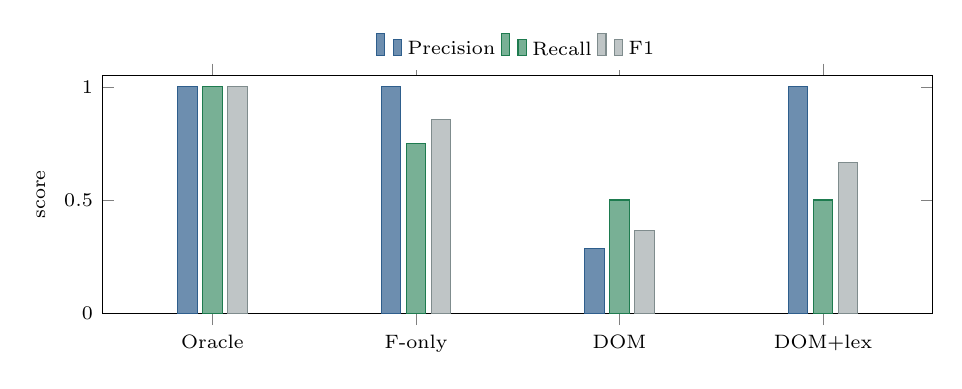
\begin{tikzpicture}
\begin{axis}[
  ybar, bar width=7pt, width=\columnwidth, height=4.6cm,
  ymin=0, ymax=1.05, ylabel={score}, ylabel style={font=\scriptsize},
  symbolic x coords={Oracle,F-only,DOM,DOM+lex},
  xtick=data, tick label style={font=\scriptsize},
  legend style={font=\scriptsize,at={(0.5,1.02)},anchor=south,legend columns=3,draw=none},
  enlarge x limits=0.18]
\addplot[fill=acc!70,draw=acc]   coordinates {(Oracle,1.00) (F-only,1.00) (DOM,0.286) (DOM+lex,1.00)};
\addplot[fill=good!60,draw=good] coordinates {(Oracle,1.00) (F-only,0.75) (DOM,0.50) (DOM+lex,0.50)};
\addplot[fill=mute!50,draw=mute] coordinates {(Oracle,1.00) (F-only,0.857) (DOM,0.364) (DOM+lex,0.667)};
\legend{Precision,Recall,F1}
\end{axis}
\end{tikzpicture}
\caption{Audit accuracy by configuration. Lexical grounding fixes precision
(required-absent false alarms) but not recall (semantic grounding of
forbidden subjects).}
\label{fig:rq2}
\end{figure}

\subsection{RQ3: Is ``required absent'' necessary?}
\label{sec:eval:rq3}
Dropping $\Req$ and auditing with the intersection $S\cap\Forb$ alone keeps
precision at 1.00 but loses V-04 (recall 0.75). No setting of the forbidden
clauses can recover it, because an absence is not an element that can
intersect anything. This is the empirical counterpart of the structural
argument in \cref{sec:model}. Accessibility obligations, consent banners, and
logout affordances are all required-absent properties.

\subsection{RQ4: Fingerprint stability and sensitivity}
\label{sec:eval:fp}
We re-render each of the six pages 50 times and inject fresh per-request noise
into every capture: \texttt{data-session}/\texttt{data-csrf} tokens, a
generated hex \texttt{id}, a \texttt{data-request-id}, a 13-digit timestamp,
and a CDP-shaped AX tree with new \texttt{nodeId}s. A naive hash of URL, DOM,
and AX produces \textbf{300 distinct states} for 6 logical pages (one per
load). $\phi$ produces exactly \textbf{6}, one per page (\cref{tab:fp}).
Normalization does not over-merge: deleting the \emph{Delete user} button from
the admin page changes its fingerprint, so a security-relevant difference
still yields a distinct state.

\begin{table}[t]
\centering\small
\caption{RQ4: distinct state ids over 50 noisy captures per page.}
\label{tab:fp}
\begin{tabular}{@{}lrr@{}}
\toprule
Page & naive hash & $\phi$ (normalized) \\
\midrule
\texttt{/index.html}            & 50 & 1 \\
\texttt{/pages/login.html}      & 50 & 1 \\
\texttt{/pages/register.html}   & 50 & 1 \\
\texttt{/pages/dashboard.html}  & 50 & 1 \\
\texttt{/pages/reports.html}    & 50 & 1 \\
\texttt{/pages/admin.html}      & 50 & 1 \\
\midrule
Total (6 logical states) & 300 & 6 \\
\multicolumn{2}{@{}l}{Real change (Delete button removed) detected?} & yes \\
\bottomrule
\end{tabular}
\end{table}

\subsection{Threats to validity}
\emph{External:} there is one small, static, hand-built application with four
planted defects. The results show the mechanism works, not that it generalises,
and \cref{sec:discussion} outlines a benchmark to address this.
\emph{Construct:} RQ1 uses an oracle perception by design. RQ2 evaluates the
deterministic channel on HTML without a live AX tree, and the VLM channel is
implemented but not evaluated here. The RQ4 noise model covers known volatile
patterns and not, for example, rotating advertisements or A/B variants.
\emph{Internal:} the lexical-grounding ablation patches the matcher's normalizer in-process
only. It measures an effect and is not a shipped change.

\section{Related Work}
\label{sec:related}

\begin{table*}[t]
\centering\footnotesize
\caption{Positioning against the closest prior work. \checkmark{} = stated
capability, $\sim$ = partial or qualified, -- = not a goal or absent. Columns:
AE autonomous exploration; CYC cyclic state graph kept; POL declarative or NL
policy; NEG ``must-not-exist'' oracle; REQ ``required-absent'' oracle; ROLE
role-scoped; MM multimodal perception; SAFE side-effect safety; GT ground truth
scored for exact recall. Cells for prior work reflect the cited papers as read
for this draft.}
\label{tab:related}
\setlength{\tabcolsep}{4pt}
\begin{tabular}{@{}llccccccccc@{}}
\toprule
Family & System & AE & CYC & POL & NEG & REQ & ROLE & MM & SAFE & GT \\
\midrule
\multirow{4}{*}{Model inference}
 & Crawljax~\cite{mesbah2012crawljax}          & \checkmark & \checkmark & -- & $\sim$ & $\sim$ & -- & -- & -- & -- \\
 & ATUSA invariants~\cite{mesbah2012invariant} & \checkmark & \checkmark & $\sim$ & \checkmark & \checkmark & -- & -- & -- & -- \\
 & WebMate~\cite{dallmeier2013webmate}         & \checkmark & $\sim$ & -- & -- & -- & $\sim$ & -- & -- & -- \\
 & Stoat / APE / DroidBot~\cite{su2017stoat,gu2019ape,li2017droidbot} & \checkmark & \checkmark & -- & -- & -- & -- & -- & -- & -- \\
\midrule
\multirow{2}{*}{Property / a11y}
 & Kea~\cite{xiong2024kea}                     & \checkmark & $\sim$ & \checkmark & $\sim$ & $\sim$ & -- & -- & -- & $\sim$ \\
 & MATE~\cite{eler2018mate}                    & \checkmark & $\sim$ & -- & $\sim$ & \checkmark & -- & -- & -- & -- \\
\midrule
\multirow{3}{*}{Access control}
 & Sun et al.~\cite{sun2011static}             & -- & $\sim$ & -- & $\sim$ & -- & \checkmark & -- & -- & -- \\
 & Li et al.~\cite{li2014blackbox}             & \checkmark & $\sim$ & -- & $\sim$ & -- & \checkmark & -- & $\sim$ & -- \\
 & BACScan~\cite{liu2025bacscan}               & \checkmark & \checkmark & -- & $\sim$ & -- & \checkmark & -- & -- & \checkmark \\
\midrule
\multirow{4}{*}{LLM/VLM testing}
 & GPTDroid / DroidAgent~\cite{liu2024gptdroid,yoon2024droidagent} & \checkmark & $\sim$ & -- & -- & -- & -- & -- & -- & -- \\
 & VisionDroid~\cite{liu2024visiondroid}       & \checkmark & $\sim$ & -- & -- & -- & -- & \checkmark & -- & $\sim$ \\
 & AXNav~\cite{taeb2024axnav}                  & -- & -- & \checkmark & $\sim$ & $\sim$ & -- & \checkmark & -- & -- \\
 & UIGuard~\cite{chen2023uiguard}              & -- & -- & $\sim$ & \checkmark & -- & -- & \checkmark & -- & $\sim$ \\
\midrule
Agent policy & ST-WebAgentBench~\cite{levy2026stwebagentbench} & -- & -- & \checkmark & $\sim$ & $\sim$ & -- & $\sim$ & $\sim$ & \checkmark \\
\midrule
\textbf{This work} & \textbf{\sys{}}                 & \checkmark & \checkmark & $\sim$ & \checkmark & \checkmark & \checkmark & $\sim$ & $\sim$ & $\sim$ \\
\bottomrule
\end{tabular}
\end{table*}

\Cref{tab:related} summarises the positioning. No prior system combines
autonomous cyclic exploration with a role-scoped oracle of both polarities.
The closest neighbours are ATUSA~\cite{mesbah2012invariant} on the oracle side
and BACScan~\cite{liu2025bacscan} on the role side.

\paragraph{Web and GUI model inference.}
GUI Ripping~\cite{memon2003ripping} and Crawljax~\cite{mesbah2012crawljax}
reverse-engineer GUIs into event-flow and state-flow graphs. WebMate
\cite{dallmeier2013webmate} generates tests for Web~2.0 applications. On
Android, Sapienz~\cite{mao2016sapienz}, Stoat~\cite{su2017stoat},
APE~\cite{gu2019ape}, DroidBot~\cite{li2017droidbot}, and
Humanoid~\cite{li2019humanoid} explore with search, stochastic models, model
refinement, or learned policies, mostly with crash oracles. These models are
cyclic by construction, so we do \emph{not} claim the cyclic graph as novel.
We claim only that the audit keeps it intact. State abstraction and
near-duplicate detection are well studied~\cite{yandrapally2020nearduplicate}.
Our fingerprint is a conventional instance, which we evaluate for stability
and sensitivity but do not claim as a contribution. Doup\'e et
al.~\cite{doupe2012enemy} infer server state machines while tracking
state-changing requests. Our claim-before-execute rule addresses the related
problem of not re-firing side effects in the auditor itself.

\paragraph{Test oracles and invariants.}
The oracle problem is surveyed by Barr et al.~\cite{barr2015oracle}. GUI
oracles check expected state after each action~\cite{memon2000oracles}. ATUSA
\cite{mesbah2012invariant} checks generic and application-specific DOM
invariants on every crawled state, and can express both presence and absence.
Expressively, then, \sys{}'s oracle adds nothing that a skilled user could not
hand-write as ATUSA invariants. Our delta is that polarity is part of a typed
policy schema, clauses range over a semantic vocabulary that is portable
across pages and markup, clauses are role-scoped, and each violation is tagged
with the operation that produced it. That tagging is what enables the
per-polarity analysis of \cref{prop:asym}. Property-based Android testing
(Kea~\cite{xiong2024kea}) and accessibility checkers (MATE~\cite{eler2018mate})
check properties or fixed rules during exploration, but without roles or
policy polarity.

\paragraph{Access-control testing.}
Sun et al.~\cite{sun2011static} derive per-role sitemaps statically. Li et
al.~\cite{li2014blackbox}, Noseevich and Petukhov~\cite{noseevich2011detecting},
MACE~\cite{monshizadeh2014mace}, BACScan~\cite{liu2025bacscan}, and
BACFuzz~\cite{dharmaadi2025bacfuzz} detect broken access control by comparing
or mutating requests across identities. These tools decide whether the
\emph{server} enforces authorization. \sys{} decides whether the \emph{UI shown
to a role} conforms to a declared policy, including a required-absent half
that request-level tools do not model. UI exposure is not in itself an OWASP
A01 vulnerability~\cite{owasp2021a01}, and we frame \sys{} as policy
conformance and least-privilege UI, complementary to request-level scanning.

\paragraph{LLM and VLM GUI agents and testers.}
GPTDroid~\cite{liu2024gptdroid}, DroidAgent~\cite{yoon2024droidagent}, and
AutoDroid~\cite{wen2024autodroid} use LLMs to explore or automate mobile apps.
VisionDroid~\cite{liu2024visiondroid} uses multimodal LLMs to detect non-crash
functional bugs. AXNav~\cite{taeb2024axnav} and
AUITestAgent~\cite{hu2024auitestagent} turn natural-language test
instructions or requirements into GUI interaction and verification, and
WebTestPilot~\cite{teoh2026webtestpilot} infers oracles from
natural-language specifications. UIGuard~\cite{chen2023uiguard} detects dark
patterns, a fixed taxonomy of \emph{forbidden} UI. Web-agent benchmarks
(WebArena~\cite{zhou2024webarena}, Mind2Web~\cite{deng2023mind2web},
OSWorld~\cite{xie2024osworld}) and SeeAct~\cite{zheng2024seeact} show that
grounding is the bottleneck for acting. ST-WebAgentBench
\cite{levy2026stwebagentbench} evaluates whether \emph{agents} comply with
policies. \sys{} instead uses policy to audit the \emph{application}. In
these systems the model typically issues the verdict. \sys{} withholds
existence and absence judgements from the model.

\paragraph{Negation and compositionality in VLMs.}
Alhamoud et al.~\cite{alhamoud2025negation} show that VLMs perform close to
chance on negated queries. ARO~\cite{yuksekgonul2023aro} and
CREPE~\cite{ma2023crepe} document bag-of-words behaviour and weak
compositionality. \Cref{prop:asym} explains why this matters specifically for
auditing. The damage a perception error does depends on the polarity of the
clause it feeds, so negation weakness is not a uniform accuracy tax.

\paragraph{From natural language to specifications.}
nl2spec~\cite{cosler2023nl2spec} and NL2LTL~\cite{fuggitti2023nl2ltl}
translate natural language into temporal logic with LLMs. \sys{}'s planned
policy compiler targets a much simpler clause language
$(\sigma,\rho,\pi)$ with a human confirmation gate. Extending it to
path-sensitive properties over the cyclic graph is where this line of work
becomes directly relevant.

\section{Discussion and Research Agenda}
\label{sec:discussion}

\paragraph{Subject grounding is the crux.}
RQ2 shows that once exploration and the audit algebra are correct, accuracy
depends on one mapping: from a policy \emph{subject} (``admin link'') to the
elements and capabilities of a rendered state. Lexical normalization closes
the easy half. The semantic half, deciding what an element \emph{is} and what
it \emph{lets the user do}, is where a VLM earns its cost, and also where
negation weakness and hallucination come in. \Cref{prop:asym} suggests
evaluating grounding \emph{separately per polarity}. A single accuracy number
hides whether a model fails in the direction that misses forbidden exposures
or in the direction that raises false alarms on required ones.

\paragraph{Proposed: three-valued, cross-checked verdicts.}
Given the asymmetry, we propose extending the audit from $\{\textsf{clean},
\textsf{violated}\}$ to a Kleene-style $\{\textsf{clean}, \textsf{violated},
\textsf{indeterminate}\}$. The verdict is \textsf{indeterminate} when the
deterministic DOM/AX channel and the VLM channel disagree on $\sigma\in\Sig(v)$.
An indeterminate forbidden clause is escalated to a human with evidence from
both channels and is never silently cleared. This turns the corollary of
\cref{prop:asym} into a routing rule instead of a tuning problem.

\paragraph{Scope predicates beyond roles.}
Clauses are currently scoped by role only. The test application shows why this
is not enough. ``Every \emph{signed-in} page must offer a logout control'' would
fire on the login page, where a logout control is correctly absent. The fix is
a page-scope predicate on clauses (for example, over URL patterns or state
properties). In the limit, that means path-sensitive properties over the
cyclic graph (``no state reachable from \emph{login} without authenticating
exposes \texttt{delete-user}''). Such properties are exactly why back-edges
must be kept.

\paragraph{Replay safety beyond action kinds.}
\Cref{prop:term} guarantees at-most-once per claimed pair, not per effect.
Restricting replay to $\{\texttt{navigate},\texttt{click},\texttt{back}\}$
excludes form fills and submissions, but it assumes that clicks are
navigational. A one-click destructive control on a replay path violates that
assumption. Candidate refinements are (i) classifying controls as mutating
from their accessible name and capability tags before they are made
replayable, (ii) snapshot-and-restore of the AUT between replays where the
deployment allows it, and (iii) multi-browser exploration that parks one
browser per frontier state, which reduces replay at the cost of memory.

\paragraph{Cross-role differential auditing.}
Because a role-gated element changes the DOM, and therefore the fingerprint,
running \sys{} once per role yields one graph per role. Aligning these graphs
by URL and action identity gives a \emph{differential} view (``what does a
guest see at this URL that only an admin should?''). That view needs no
hand-written forbidden list, and we plan to add it as a reporting-layer
analysis.

\paragraph{Towards a benchmark.}
To move beyond one application, we propose \textsc{NegUI}, a benchmark of
seeded applications. Each ships \texttt{app.json}, \texttt{policy.json}, and
\texttt{violations.json}, and violations are stratified by clause type
(forbidden-present vs.\ required-absent), by grounding difficulty (lexical,
semantic, visual-only), and by depth. Planned seeds include the existing
RBAC, feature-flag, and consent-banner demos in the repository. Scoring is
exact-set agreement, reported per polarity.

\section{Conclusion}
\label{sec:conclusion}

\sys{} audits what a role can \emph{see}, where workflow tests check what a
user can \emph{do}. Formalising the policy oracle as two typed set operations
makes absence a first-class violation. It also exposes a structural fact:
perception errors propagate in opposite directions for forbidden and required
clauses, so no single perception bias is safe for both. On a polarity-complete
ground-truth application, the exploration loop and audit algebra are exact
when perception is an oracle. The deterministic perception channel shows the
predicted asymmetry, and a lexical-grounding ablation isolates semantic
subject grounding as the open problem.

The next steps follow directly:
(i)~run the pipeline end to end with the live Playwright crawler and the
deterministic and VLM perception channels;
(ii)~evaluate presence and absence judgements separately per polarity on a
probe set of hard cases (unlabelled \texttt{<div>} controls, hidden and
icon-only elements);
(iii)~add page-scope predicates and three-valued verdicts;
(iv)~narrow replay safety beyond action kinds; and
(v)~release \textsc{NegUI} with a Crawljax-plus-invariants baseline.

\paragraph{Artifact.}
The code, the ground-truth applications, and the scripts that produce every
number in this paper are in the project repository
(\nolinkurl{docs/report/experiments/}).


\balance
\bibliographystyle{unsrtnat}
\bibliography{references}

\end{document}
